%----------------------------------------------------
% Setup Beamer
%----------------------------------------------------
\documentclass[hyperref={colorlinks=true}]{beamer}

%----------------------------------------------------
% Packages to use
%----------------------------------------------------
\input{../packages.sty}

%----------------------------------------------------
% Setup Theme
%----------------------------------------------------
\input{../theme.sty}

%----------------------------------------------------
% Table of Contents at each section transition
%----------------------------------------------------

\AtBeginSection[]
{
   \begin{frame}
       \frametitle{Outline}
       \setcounter{tocdepth}{2}
       \tableofcontents[currentsection]
   \end{frame}
}

%----------------------------------------------------
% Colors
%----------------------------------------------------
\input{../mycolors.sty}

%----------------------------------------------------
% Style, formatting, and new commands
%----------------------------------------------------
\input{../../global.sty}
\input{../newcommands.sty}
\input{../EandMcommands.sty}

%----------------------------------------------------
% Set paths for plots and images
%----------------------------------------------------
\input{../paths.sty}

%----------------------------------------------------
% SETTINGS FOR THIS LECTURE
%----------------------------------------------------
\newcommand{\lecnum }  {Lecture 10}
\newcommand{\lecdate}  {October 31, 2018}
\newcommand{\topic}    {Newton's method for ODEs!}

%-----------------------------------------------------------------------------------------
% Title: [Column]{Title}
%-----------------------------------------------------------------------------------------
\title[PHYS 250 (Autumn 2019) -- \lecnum]{\topic}

%-----------------------------------------------------------------------------------------
% SubTitle: [Column]{Subtitle}
%-----------------------------------------------------------------------------------------
\subtitle{PHYS 250 (Autumn 2019) -- \lecnum}

%-----------------------------------------------------------------------------------------
% Author: [SubAuthor]{Author}
%-----------------------------------------------------------------------------------------
\author[D.W.~Miller]{David Miller}

%----------------------------------------------------
% Institute: [SubInst]{Institute}
%----------------------------------------------------
\institute[EFI, Chicago] 
{
  Department of Physics and the Enrico Fermi Institute\\
  University of Chicago
}

%----------------------------------------------------
% Institute: [SubInst]{Institute}
%----------------------------------------------------
\date[\lecdate]{\lecdate}

\subject{PHYS 250 Lecture}

\begin{document}

%==========================================================================================
% TITLE PAGE
%==========================================================================================

{
\begin{frame}
  \titlepage
\end{frame}
}

%==========================================================================================
\section[Reminders]{Reminders}
%==========================================================================================

%-----------------------------------------------------------------------------------------
\subsection[Reminders from Lecture 9]{Reminders from Lecture 9}
%-----------------------------------------------------------------------------------------

\begin{frame}%[shrink=10]
  \frametitle{Reminders from last time}

  Looked at one of two primary and exemplary methods for root finding, which is part of the foundation of optimization and differential equation solving.
  
  \vspace{0.3cm}
  
  \begin{ucblock}{Fundamental root finding methods}
    \begin{itemize}
      \item \bluebf{Bisection method (aka ``incremental search''):} (Tuesday)
      \begin{itemize}
        \item \textbf{PROs:} exceptionally simple and requires no knowledge of the function whose roots are sought
        \item \textbf{CONs:} doesn't use the potentially very useful knowledge of the roots that are sought
      \end{itemize}
      \item \alertbf{Newton's Method:} (today)
      \begin{itemize}
        \item \textbf{PROs:} converges much faster than bisection
        \item \textbf{CONs:} requires a calculation or estimation of the first derivative of the function
      \end{itemize}
    \end{itemize}
  \end{ucblock}
  
  Today, we will expand on Newton's method and go several steps further.

\end{frame}

%-----------------------------------------------------------------------------------------
\subsection[Newton's method]{Newton's method}
%-----------------------------------------------------------------------------------------

\begin{frame}%[shrink=10]
  \frametitle{Newton's method (I)}

  The fundamental form of the method alluded to in the last lecture is \bluebf{Newton's method}. The core of this approach is to use information about the function in order to inform how \bluebf{big} of a step size to take with each iteration.
  
  \mysp
  
  Suppose a function $F(x)$ has a root $ x = x_0$ and you are within $\delta$ of that root at $x = x_0 - \delta$. The question we want to answer is: 
  
  \mysp
  
  \begin{ucblock}{}
    How far away from the root are we actually? What is the value of $\delta$?
  \end{ucblock}
  
  \mysp
  
  Using a Taylor expansion (as Wah told us!) 
  
  \begin{equation}
    F(x_0) = F(x+\delta) \approx F(x) + \delta F^{\prime}(x) + \frac{1}{2}\delta^2 F^{\prime\prime}(x) + \mathcal{O}(\delta^3)
  \end{equation}
  
  By setting $F(x_0) = 0$ by assumption, we can make the linear approximation to $\delta \approx \Delta$ as
  
  \begin{equation}
    \Delta = - \frac{F(x)}{F^{\prime}(x)}
  \end{equation}
  
\end{frame}

%-----------------------------------------------------------------------------------------

\begin{frame}%[shrink=10]
  \frametitle{Newton's method (II)}

  Therefore, we can choose a starting point $x_i$ and then update $x$ according to Newton
  
  \mysp
  
  \begin{equation}
    x_{i+1} = x_{i} - \frac{F(x_i)}{F^{\prime}(x_i)}
  \end{equation}
  
  The iteration stops after $j$ iterations when 
  
  \begin{equation}
   | x - x_j | \leq \epsilon
  \end{equation}  
\end{frame}

%-----------------------------------------------------------------------------------------

\begin{frame}%[shrink=10]
  \frametitle{Precision of Newton's method}

  \begin{columns}
  
    \column{0.5\textwidth}
   
      For any estimate $x_i$ of the method, the error, $E_i$ is the difference between the true root $x$ and the estimate:
      
      \begin{equation}
        E_i = x - x_i
      \end{equation}
   
      Merely by inspecting the design of Newton's method, you can see that the precision of the estimate for a subsequent iteration will be given by
      %
      \begin{eqnarray}
        E_{i+1} &=& E_i + \frac{F(x)}{F^{\prime}(x)} \\
                &=& -\frac{F^{\prime\prime}(x)}{2F^{\prime}(x)}E_i^2
      \end{eqnarray}
   
    \column{0.5\textwidth}
    
      \begin{figure}
        \centering
        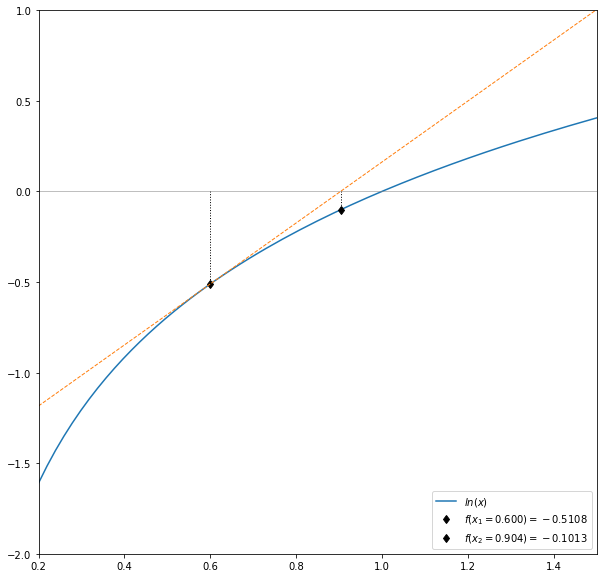
\includegraphics[width=\columnwidth]{NewtonsMethodExample-lnx.png}
      \end{figure}
    
  \end{columns}

\end{frame}

%-----------------------------------------------------------------------------------------

\begin{frame}%[shrink=10]
  \frametitle{Convergence of Newton's method}

  \begin{columns}
  
    \column{0.5\textwidth}
   
      Consequently, Newton's method \bluebf{converges quadratically}
      \begin{itemize}
        \item the error is the square of the error in the previous step)
        \item the number of significant figures is roughly doubled in every iteration, provided that $x_i$ is \alertbf{sufficiently} close to the root.
      \end{itemize} 
         
      However, a critical assumption is that $F^{\prime}(x) \neq 0$; for all $x \in I$, where $I$ is the interval $[x - r, x + r]$ for some $r \geq |x - x_0|$ and $x$ is the true root and $x_0$ was the starting point.
         
    \column{0.5\textwidth}
    
      \begin{figure}
        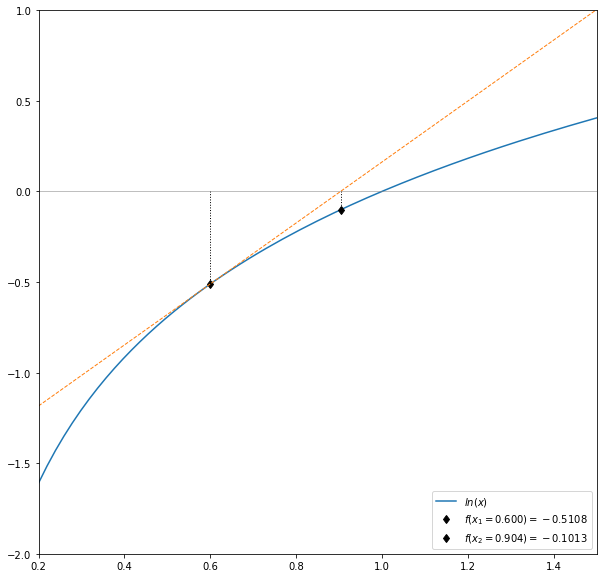
\includegraphics[width=\columnwidth]{NewtonsMethodExample-lnx.png}
      \end{figure}
    
  \end{columns}

\end{frame}


%-----------------------------------------------------------------------------------------

\begin{frame}%[shrink=10]
  \frametitle{Pathologies and divergent scenarios}

  \setbeamercovered{transparent}

  \begin{columns}
  
    \column{0.5\textwidth}
   
      That is definitely not always the case. Let's look at a pathological example. Here is a fun mystery function that I cooked up (since you need to do something similar on your homework):
      
      \begin{itemize}[<+->]
         \item $x_0 = 2.000$, \bluebf{7 iterations}
         \item $x_0 = -2.000$, \bluebf{2 iterations}
         \item $x_0 = 3.000$, \bluebf{2 iterations}
         \item $x_0 = -1.214$, \bluebf{4 iterations}
         \item Slight modification: $x_0 = -1.213$, \alertbf{no convergence}
         \item Slight modification: $x_0 = 3.000$, \alertbf{no convergence}
      \end{itemize}  
         
    \column{0.5\textwidth}
      
      \begin{figure}
        \centering
        \foreach \n in {1,...,6}%
          {\includegraphics<\n>[width=0.95\columnwidth]{NewtonsMethodExample-Pathology\n.png}}
      \end{figure}
    
  \end{columns}

\end{frame}

%-----------------------------------------------------------------------------------------

\begin{frame}%[shrink=10]
  \frametitle{Backtracking}

  In the last examples above we have a case where the search falls into the pathology of a situation where the initial guess was not \alertbf{sufficiently close} to the root. an ``infinite'' loop without ever getting there. 
  
  \mysp
  
  A solution to this problem is called \alertbf{backtracking}. 
  
  \mysp
  
  \begin{ucblock}{Backtracking}
    In cases where the new guess $x_0 + \Delta x$ leads to an increase in the magnitude of the function, $|f(x_0 + \Delta x)|^{2} > |f(x_0)|^{2}$, you should backtrack somewhat and try a smaller guess, say, $x_0 + \Delta x/2$. If the magnitude of $f$ still increases, then you just need to backtrack some more, say, by trying $x_0 + \Delta x/4$ as your next guess, and so forth.
  \end{ucblock}

\end{frame}

%-----------------------------------------------------------------------------------------

\begin{frame}%[shrink=10]
  \frametitle{Pathological case fixed with backtracking}

  \setbeamercovered{transparent}

  \begin{columns}
  
    \column{0.5\textwidth}
   
      Fixing the pathological example with backtracking:
      
      \begin{itemize}[<+->]
         \item $x_0 = -1.213$, \alertbf{no convergence}
         \item $x_0 = 3.000$, \alertbf{no convergence}
         \item $x_0 = 1.500$, \bluebf{3 iterations}
      \end{itemize}  
         
    \column{0.5\textwidth}
      
      \begin{figure}
        \centering
        \includegraphics<1>[width=0.95\columnwidth]{NewtonsMethodExample-Pathology5.png}
        \includegraphics<2>[width=0.95\columnwidth]{NewtonsMethodExample-Pathology6.png}
        \includegraphics<3>[width=0.95\columnwidth]{NewtonsMethodExample-Pathology7.png}
      \end{figure}
    
  \end{columns}

\end{frame}

%-----------------------------------------------------------------------------------------
\subsection[System of equations]{System of equations}
%-----------------------------------------------------------------------------------------

\begin{frame}%[shrink=10]
  \frametitle{Multidimensional problems}

  Up to this point, we have confined our attention to solving the single equation $F(x) = 0$. Let us now consider the $n$-dimensional version of the same problem, namely
  
  \begin{equation}
    \vec{F}(\vec{x}) = 0
  \end{equation}

  where we allow for a vector of functions $\vec{F} = \{f_1(\vec{x}), f_2(\vec{x}), ..., f_n(\vec{x})\}$, and $\vec{x} = \{ x_1, x_2, ..., x_{n} \}$.
  
  \mysp
  
  The solution of $n$ simultaneous, nonlinear equations is a much more formidable task than finding the root of a single equation. The trouble is the lack of a reliable method for bracketing the solution vector $\vec{x}$. Therefore, we cannot always provide the solution algorithm with a good starting value of $x$, unless such a value is suggested by the physics of the problem.
  
  \mysp
  
  Newton's method is the workhorse here!
  

\end{frame}

%-----------------------------------------------------------------------------------------

\begin{frame}%[shrink=10]
  \frametitle{Reminder of the general problem}

  Start by considering each one of the $n$ functions, $f_n(x)$, separately:

  \begin{eqnarray}
    f_i(\vec{x}) &=& f_i(\vec{a} )+ \sum_j^n \frac{\partial f_i}{\partial x_j}|_{\vec{x}} \Delta x_j + \frac{1}{2!} \sum_j^n \sum_k^n \frac{\partial^2 f_i}{\partial_j \partial_k}|_{\vec{x}} \Delta x_j \Delta x_k \\
                 %
                 &=& f_i(\vec {a} )+ \Delvec f_i(\vec{a}) \cdot \vec{\Delta x} + \frac{1}{2!}\vec{\Delta x}^{\mathrm {T} }\mathbf {H} (\vec{a})\vec{\Delta x}
  \end{eqnarray}
  
  where $\mathbf {H}$ is the \bluebf{Hessian matrix}, describing the \alertbf{curvature} of $f_i(\vec{x})$ by
  
  \begin{equation}
    {\mathbf {H} }_{j,k}={\frac {\partial ^{2}f(\vec{a})}{\partial x_{j}\partial x_{k}}}
  \end{equation}
  
  (The determinant of $\mathbf {H}$ is also sometimes referred to as \alertbf{the Hessian}) and $\vec{\Delta x}$ is a vector that describes the distance from the point about which we are expanding the function $f_i(\vec{x})$.

\end{frame}

%-----------------------------------------------------------------------------------------

\begin{frame}%[shrink=10]
  \frametitle{Specific example (I)}

  Let's take a very explicit example of a function:

  \begin{equation}
    f(\vec{x}) = f(x, y) = \ln \sqrt{x^2 + y^2} 
  \end{equation}
  
  and compute the gradient and Hessian matrix at $x=-2, y=1$ (see point on graph below).
    
  \begin{figure}
    \centering
    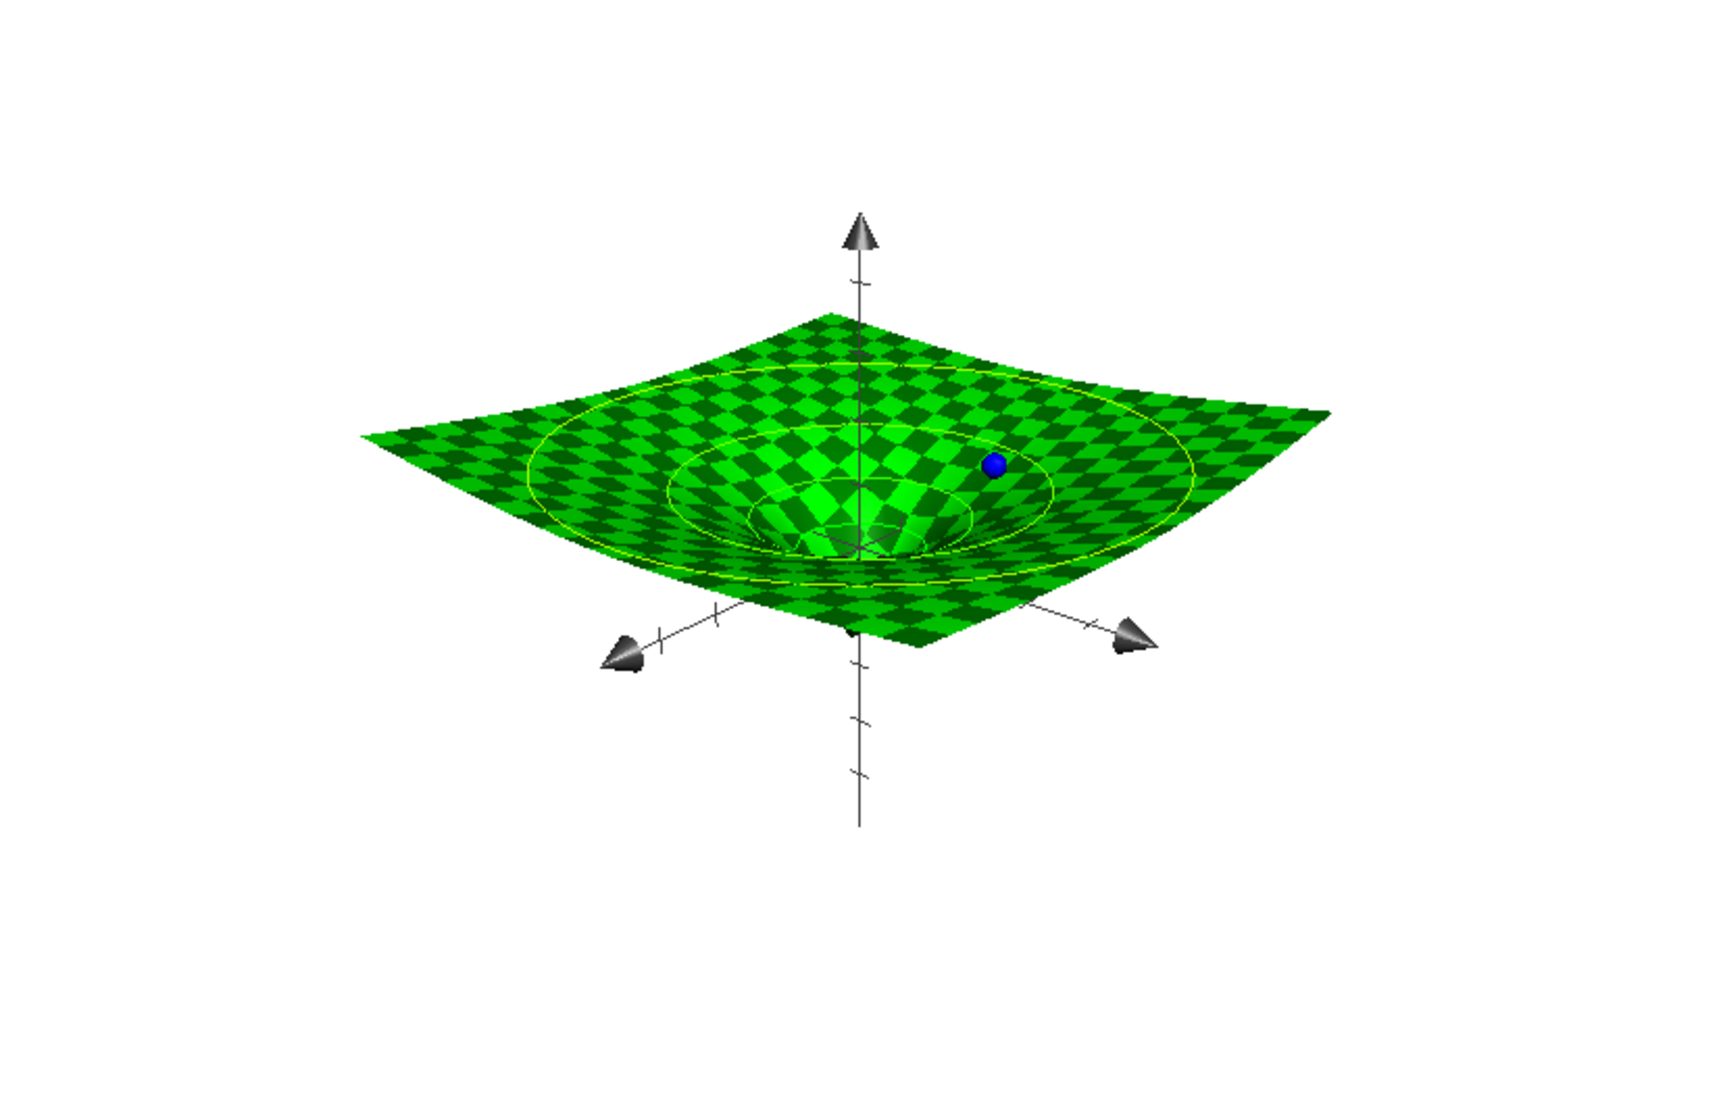
\includegraphics[width=0.65\columnwidth]{Function1-checkerboard.pdf}
  \end{figure}

\end{frame}

%-----------------------------------------------------------------------------------------

\begin{frame}%[shrink=10]
  \frametitle{Specific example (II)}

  First, we calculate the gradient:
  %
  \begin{eqnarray}
    \partialx{f} &=& \frac{1}{\sqrt{x^2 + y^2}} \left( \frac{1}{2} \frac{2x}{\sqrt{x^2 + y^2}}  \right) \\
                 &=& \frac{x}{x^2 + y^2} \\
    \partialy{f} &=& \frac{y}{x^2 + y^2}
  \end{eqnarray}
  %
  Therefore
  %
  \begin{equation}
    \Delvec f(x,y) = (\frac{x}{x^2 + y^2} , \frac{y}{x^2 + y^2})
  \end{equation}
  %
  Or, in matrix notation
  %
  \begin{equation}
    \Delvec f(x,y) = \left[\begin{array}{c}
                             \frac{x}{x^2 + y^2} \\
                             \frac{y}{x^2 + y^2}
                           \end{array}\right], 
    %                       
    \Delvec f(-2,1) = \left[\begin{array}{c}
                             -0.4 \\
                             0.2
                           \end{array}\right]                     
  \end{equation}

\end{frame}

%-----------------------------------------------------------------------------------------

\begin{frame}%[shrink=10]
  \frametitle{Specific example (III)}

  \begin{figure}
    \centering
    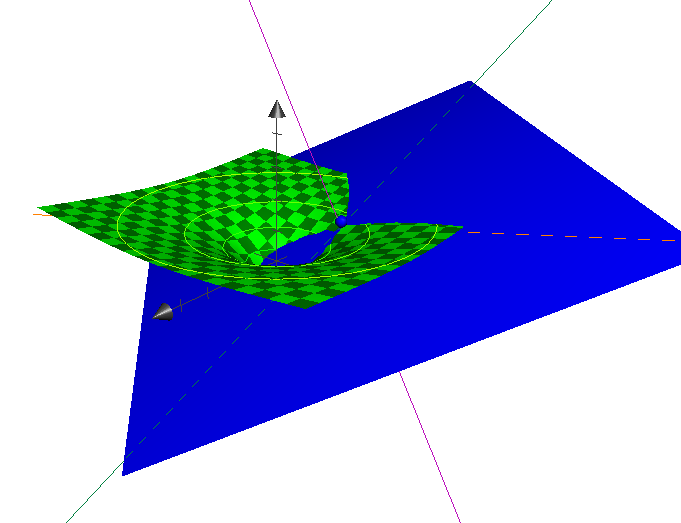
\includegraphics[width=0.85\columnwidth]{Function1-plane.png}
  \end{figure}

\end{frame}

%-----------------------------------------------------------------------------------------

\begin{frame}%[shrink=10]
  \frametitle{Specific example (IV)}

  Next, we calculate the Hessian matrix:
  %
  \begin{eqnarray}
    \partialxsq{f}  &=& \frac{(x^2 + y^2) - x(2x)}{(x^2 + y^2)^2} \\
                    &=& \frac{-x^2 + y^2}{(x^2 + y^2)^2} \\
    \partialysq{f}  &=& \frac{x^2 - y^2}{(x^2 + y^2)^2} \\
    \partialxysq{f} &=& \partialxysq{f} = \frac{-2xy}{(x^2 + y^2)^2}
  \end{eqnarray}
  %
  Therefore
  %
  \begin{equation}
    \mathbf {H}     = \left[\begin{array}{c c}
                             -x^2 + y^2 & -2xy \\
                             -2xy       & x^2 - y^2
                           \end{array}\right] \frac{1}{(x^2 + y^2)^2} , 
    %                       
    \mathbf {H}     = \left[\begin{array}{c c}
                             -0.12 & 0.16 \\
                             0.16  & 0.12
                           \end{array}\right]                    
  \end{equation}

\end{frame}


%-----------------------------------------------------------------------------------------

\begin{frame}%[shrink=10]
  \frametitle{Jacobian matrix}

  In the case that the function $F$ is a vector of functions, $\vec{F} = \{f_1(\vec{x}), f_2(\vec{x}), ..., f_n(\vec{x})\}$ (i.e. a system of equations) then the gradient \alertbf{also has a name:} \bluebf{Jacobian}.
  
  \begin{equation}
    \mathbf {J} = \left[ \partialxone{\vec{f}} \, \cdots \, \partialxn{\vec{f}} \right]%
                = \left[ \begin{array}{c c c}
                             \partialxone{f_1} & \cdots & \partialxn{f_1} \\
                             \vdots            & \ddots & \vdots \\
                             \partialxone{f_n} & \cdots & \partialxn{f_n} 
                           \end{array}\right]
  \end{equation}
  

  \begin{equation}
    \mathbf{J}_{ij}= \partialxj{f_i}
  \end{equation}

  The Jacobian matrix is important because if the function $\vec{f}$ is differentiable at a point $\vec{x}$, then $\mathbf{J}$ defines a linear map which is the best (pointwise) linear approximation of the function $\vec{f}$ near the point $\vec{x}$.
  
  \centering \bluebf{That's exactly what we want!}

\end{frame}

%-----------------------------------------------------------------------------------------

\begin{frame}%[shrink=10]
  \frametitle{Newton's method for a system of equations}

  The following steps constitute Newton's method for simultaneous, nonlinear equations:
  
  \begin{enumerate}
    \item Estimate the solution vector $\vec{x}$
    \item Evaluate $\vec{f}(\vec{x})$
    \item Compute the Jacobian matrix $\mathbf{J}$ ($J_{ij}$)
    \item Setup the simultaneous equations $\mathbf{J}(\vec{x}) \vec{\Delta x} = - \vec{f}(\vec{x})$  and solve for $\vec{x}$
    \item Let $\vec{x}\leftarrow \vec{x} + \vec{\Delta x}$ and repeat steps 2-5
  \end{enumerate}

\end{frame}



%-----------------------------------------------------------------------------------------

\begin{frame}%[shrink=10]
  \frametitle{Comments on matrix computing and manipulations}

  Physical systems are often modeled by systems of simultaneous equations, and it is very convenient to write these matrix form. In fact, several physical systems can be expressed this way very conveniently.
  
  \vspace{0.3cm}
  
  \begin{itemize}
    \item Physical optics (lenses, mirrors, etc)
    \item Electromagnetic waves propagating near boundaries and in matter
    \item Quantum mechanical systems
    \item Classical mechanical dynamical systems
    \item etc, etc
  \end{itemize}
  
  As the models are made more realistic, the matrices often become large, and comput- ers become an excellent tool for solving such problems.

\end{frame}

%-----------------------------------------------------------------------------------------

\begin{frame}%[shrink=10]
  \frametitle{Example: weights and strings (I)}

  \begin{figure}
    \centering
    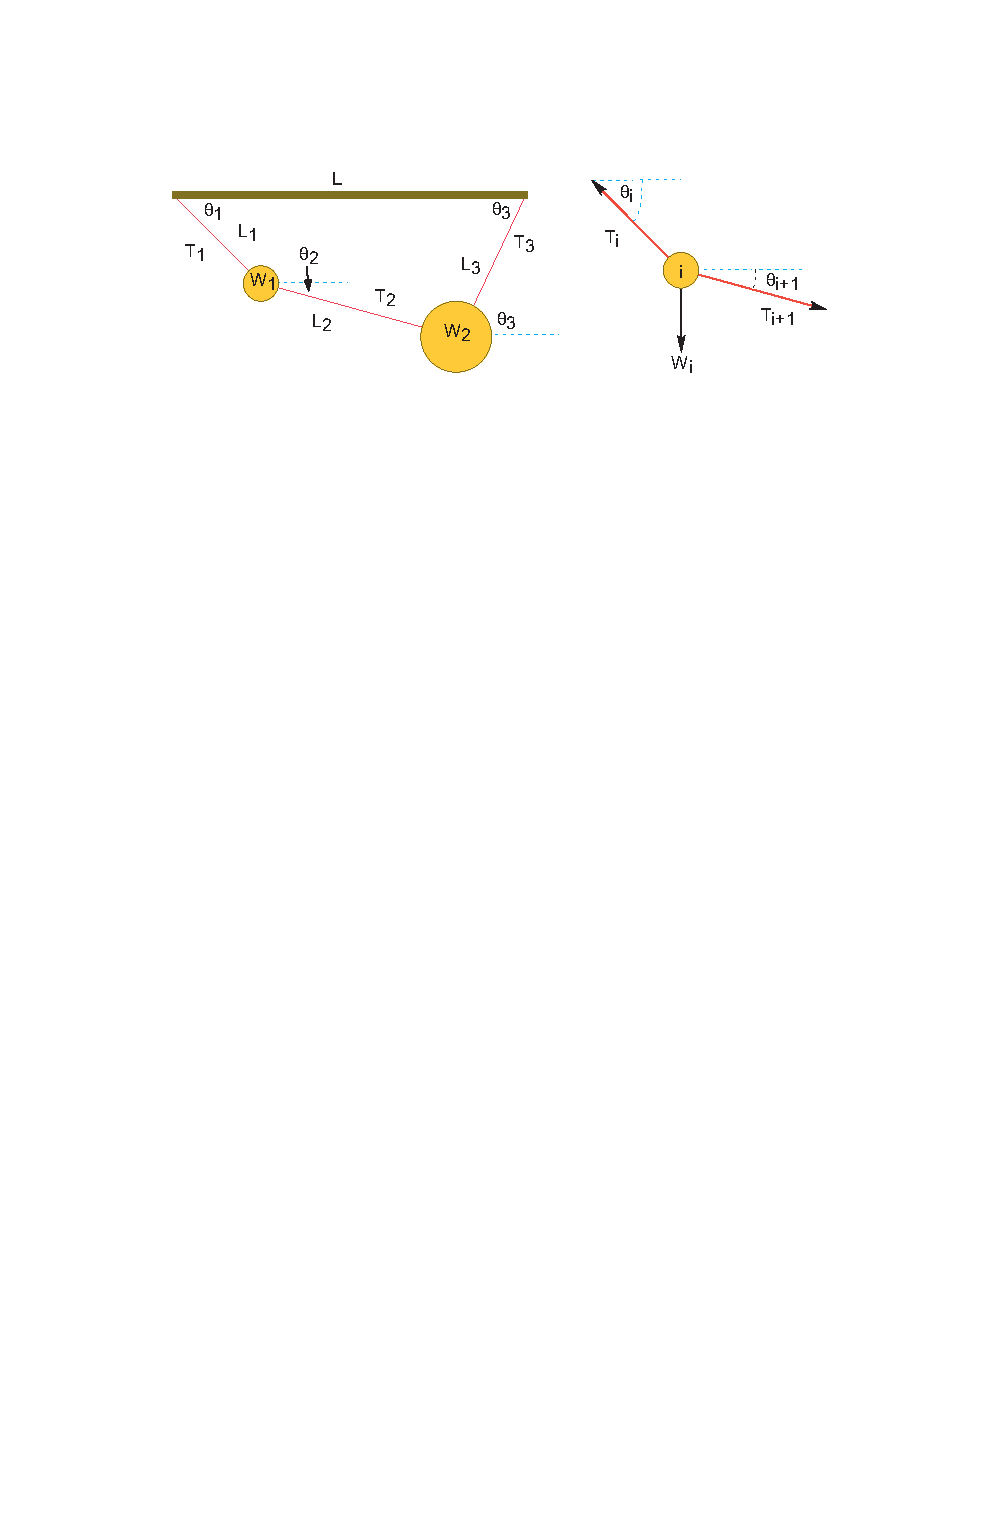
\includegraphics[width=0.85\columnwidth]{WeightsStrings.pdf}
  \end{figure}
  
  Two weights $(W_1, W_2) = (10, 20)$ are hung from three pieces of string with lengths $(L_1, L_2, L_3) = (3, 4, 4)$ and a horizontal bar of length $L = 8$. 
  
  \mysp
  
  We want to find the angles assumed by the strings and the tensions exerted by the strings.
 
  
\end{frame}

%-----------------------------------------------------------------------------------------

\begin{frame}%[shrink=10]
  \frametitle{Example: weights and strings (II)}

  The first 5 equations implement the geometric constraints that the horizontal length of the structure is $L$ and that the strings begin and end at the same height.
  %
  \begin{eqnarray}
    L_1 \cos\theta_1 + L_2 \cos\theta_2 + L_3 \cos\theta_3 &=& L \\
    L_1 \sin\theta_1 + L_2 \sin\theta_2 - L_3 \sin\theta_3 &=& 0 \\
    \sin^2 \theta_1 + \cos^2 \theta_1                      &=& 1 \\
    \sin^2 \theta_2 + \cos^2 \theta_2                      &=& 1 \\
    \sin^2 \theta_3 + \cos^2 \theta_3                      &=& 1
  \end{eqnarray}
  %
  The last three equations include trigonometric identities as independent equations because we are treating $\sin\theta$ and $\cos\theta$ as independent variables; this makes the search procedure easier to implement.
  
\end{frame}


%-----------------------------------------------------------------------------------------

\begin{frame}%[shrink=10]
  \frametitle{Example: weights and strings (III)}

  The basics physics says that since there are no accelerations, the sum of the forces in the horizontal and vertical directions must equal zero.
  %
  \begin{eqnarray}
    T_1 \sin\theta_1 - T_2 \sin\theta_2 - W_1              &=& 0 \\
    T_1 \cos\theta_1 - T_2 \cos\theta_2                    &=& 0 \\
    T_2 \sin\theta_2 + T_3 \sin\theta_3 - W_2              &=& 0 \\
    T_2 \cos\theta_2 - T_3 \cos\theta_3                    &=& 0  
  \end{eqnarray}

  Here $W_i$ is the weight of mass $i$ and $T_i$ is the tension in string $i$. Note that since we do not have
a rigid structure, we cannot assume the equilibrium of torques.
  
  \mysp
  
  These equations represent nine simultaneous nonlinear equations. While linear equations can be solved directly, nonlinear equations cannot.

\end{frame}

%-----------------------------------------------------------------------------------------

\begin{frame}%[shrink=10]
  \frametitle{Example: weights and strings (IV)}

  We apply to our set the same Newton's method algorithm as used to solve a single equation by renaming the nine unknown angles and tensions as the components of our vector $\vec{x}$ and placing the variables together as a vector:
  %
  \begin{equation}
    \vec{x} = \left[\begin{array}{c}
                      x_1 \\
                      x_2 \\
                      x_3 \\
                      x_4 \\
                      x_5 \\
                      x_6 \\
                      x_7 \\
                      x_8 \\
                      x_9        
                    \end{array}\right]
    %                       
             = \left[\begin{array}{c}
                       \sin\theta_1 \\
                       \sin\theta_2 \\
                       \sin\theta_3 \\
                       \cos\theta_1 \\
                       \cos\theta_2 \\
                       \cos\theta_3 \\
                       T_1 \\
                       T_2 \\
                       T_3
                     \end{array}\right]  \nonumber                   
  \end{equation}

\end{frame}

%-----------------------------------------------------------------------------------------

\begin{frame}%[shrink=10]
  \frametitle{Example: weights and strings (V)}

  The nine equations to be solved are written in a general form with zeros on the right-hand sides and placed in a vector:
  %
  \begin{equation}
    \vec{f(\vec{x}}) = \left[\begin{array}{c}
                      f_1(\vec{x}) \\
                      f_2(\vec{x}) \\
                      f_3(\vec{x}) \\
                      f_4(\vec{x}) \\
                      f_5(\vec{x}) \\
                      f_6(\vec{x}) \\
                      f_7(\vec{x}) \\
                      f_8(\vec{x}) \\
                      f_9(\vec{x})        
                    \end{array}\right]
    %                       
             = \left[\begin{array}{c}
                       L_1 x_4 + L_2 x_5 + L_3 x_6 - 8 \\
                       L_1 x_1 + L_2 x_2 - L_3 x_3 \\
                       x_7 x_1 - x_8 x_2 - W_1 \\
                       x_7 x_4 - x_8 x_5 \\
                       x_8 x_2 + x_9 x_3 - W_2\\
                       x_8 x_5 - x_9 x_6 \\
                       x_1^2 + x_4^2 - 1 \\
                       x_2^2 + x_5^2 - 1 \\
                       x_3^2 + x_6^2 
                     \end{array}\right]  
    %                       
             = \left[\begin{array}{c}
                       3x_4 + 4x_5 +4x_6 - 8 \\
                       3x_1 + 4x_2 - 4x_3 \\
                       x_7 x_1 - x_8 x_2 - 10 \\
                       x_7 x_4 - x_8 x_5 \\
                       x_8 x_2 + x_9 x_3 - 20 \\
                       x_8 x_5 - x_9 x_6 \\
                       x_1^2 + x_4^2 - 1 \\
                       x_2^2 + x_5^2 - 1 \\
                       x_3^2 + x_6^2 
                     \end{array}\right] \nonumber                 
  \end{equation}

  And this is then solved by computing the Jacobian and using Newton's method as usual!

\end{frame}
%
%
%%-----------------------------------------------------------------------------------------
%\subsection[Numerical differentiation]{Numerical differentiation}
%%-----------------------------------------------------------------------------------------
%
%\begin{frame}%[shrink=10]
%  \frametitle{Finite forward difference approximation (I)}
%
%    Numerical differentiation is related to interpolation: one means of finding the derivative is to approximate the function locally by a polynomial and then differentiate it. I am not going to go into detail about that, since, well, that's about the sum of it.
%
%  \mysp
%  
%  What we will discuss in a bit more detail are the \bluebf{finite difference approximations}, which, again, depend on your favorite series, \alertbf{the Taylor series}. Writing down the Taylor series' for a few definitions of the expansion parameter $h$, we have:
%  %
%  \begin{eqnarray}
%    f(x+h) &=& f(x) + hf^{\prime}(x) + \frac{h^2}{2!}f^{\prime\prime}(x) + \frac{h^3}{3!}f^{\prime\prime\prime}(x)+\frac{h^4}{4!}f^{\prime\prime\prime\prime}(x) + \cdots \nonumber \\
%    f(x-h) &=& f(x) - hf^{\prime}(x) + \frac{h^2}{2!}f^{\prime\prime}(x) - \frac{h^3}{3!}f^{\prime\prime\prime}(x)+\frac{h^4}{4!}f^{\prime\prime\prime\prime}(x) - \cdots \nonumber 
%  \end{eqnarray}
%  %
%  This leads to your favorite definition:
%  %
%  \begin{equation}
%    f^{\prime}(x) = \frac{f(x+h) - f(x)}{h} - \frac{h}{2}f^{\prime\prime}(x) - \frac{h^2}{6}f^{\prime\prime\prime}(x) - \frac{h^3}{4!}f^{\prime\prime\prime\prime}(x) + \cdots \nonumber 
%  \end{equation}
%  
%
%\end{frame}
%
%%-----------------------------------------------------------------------------------------
%
%\begin{frame}%[shrink=10]
%  \frametitle{Finite forward difference approximation (II)}
%
%  If we keep only the first terms, then we have the approximation
%  %
%  \begin{equation}
%    f^{\prime}(x) = \frac{f(x+h) - f(x)}{h} + \mathcal{O}(h)  
%  \end{equation}
%  %
%  where the truncation error is $\mathcal{O}(h)$. 
%  
%  \mysp
%  
%  \centering \alertbf{Can we do better?}
%
%\end{frame}
%
%
%%-----------------------------------------------------------------------------------------
%
%\begin{frame}%[shrink=10]
%  \frametitle{Finite central difference approximation (I)}  
%  
%  \bluebf{Yes!}, we can do significantly better than the \alertbf{finite forward difference approximation} with just a little bit of cleverness.
%  
%  \mysp
%  
%  Let's write down the definitions of the Taylor series' again for a few more definitions of the expansion parameter $h$:
%  %
%  \begin{eqnarray}
%    f(x+h) &=& f(x) + hf^{\prime}(x) + \frac{h^2}{2!}f^{\prime\prime}(x) + \frac{h^3}{3!}f^{\prime\prime\prime}(x)+\frac{h^4}{4!}f^{\prime\prime\prime\prime}(x) + \cdots \nonumber \\
%    f(x-h) &=& f(x) - hf^{\prime}(x) + \frac{h^2}{2!}f^{\prime\prime}(x) - \frac{h^3}{3!}f^{\prime\prime\prime}(x)+\frac{h^4}{4!}f^{\prime\prime\prime\prime}(x) - \cdots \nonumber \\
%    f(x+2h) &=& f(x) + 2hf^{\prime}(x) + \frac{(2h)^2}{2!}f^{\prime\prime}(x) + \frac{(2h)^3}{3!}f^{\prime\prime\prime}(x)+\frac{(2h)^4}{4!}f^{\prime\prime\prime\prime}(x) + \cdots \nonumber \\
%    f(x-2h) &=& f(x) - 2hf^{\prime}(x) + \frac{(2h)^2}{2!}f^{\prime\prime}(x) - \frac{(2h)^3}{3!}f^{\prime\prime\prime}(x)+\frac{(2h)^4}{4!}f^{\prime\prime\prime\prime}(x) - \cdots \nonumber
%  \end{eqnarray}
%
%\end{frame}
%
%%-----------------------------------------------------------------------------------------
%
%\begin{frame}%[shrink=10]
%  \frametitle{Finite central difference approximation (II)}
%
%  Putting this together we can form useful sums and differences:
%  %
%  \begin{eqnarray}
%    f(x+h) + f(x-h)   &=& 2f(x) + h^2f^{\prime\prime}(x) + \frac{h^4}{12}f^{\prime\prime\prime\prime}(x) + \cdots \nonumber \\
%    f(x+h) - f(x-h)   &=& 2hf^{\prime}(x) + \frac{h^3}{3}f^{\prime\prime\prime}(x) +  \cdots \nonumber \\
%    f(x+2h) + f(x-2h) &=& 2f(x) + 4h^2f^{\prime\prime}(x) + \frac{4h^4}{3}f^{\prime\prime\prime\prime}(x) + \cdots \nonumber \\
%    f(x+2h) - f(x-2h) &=& 4hf^{\prime}(x) + \frac{8h^3}{3}f^{\prime\prime\prime}(x) + \cdots \nonumber
%  \end{eqnarray}
%  %
%  Note that the sums contain only even derivatives, whereas the differences retain just the odd derivatives, and \alertbf{the local error is at most $\mathcal{O}(h^2)$, and is $\mathcal{O}(h^3)$ for odd powers (i.e. differences)}.
%  
%  \mysp
%  
%  These equations can be viewed as simultaneous equations that can be solved for various derivatives of $f(x)$. The number of equations involved and the number of terms kept in each equation depend on the order of the derivative and the desired degree of accuracy.
%
%\end{frame}
%
%%==========================================================================================
%\section[Initial value problems in ODEs]{Initial value problems in ODEs}
%%==========================================================================================
%
%%-----------------------------------------------------------------------------------------
%\subsection[Statement of the problem]{Statement of the problem}
%%-----------------------------------------------------------------------------------------
%
%\begin{frame}%[shrink=10]
%  \frametitle{General form and structure of ODEs}
%
%  The general form of a first-order differential equation is
%  %
%  \begin{equation}
%    y^{\prime} = f(x,y)
%  \end{equation}
%  %
%  where $y^{\prime} = \frac{dy}{dx}$ and $f(x, y)$ is a given function. The solution of this equation contains an arbitrary constant (the constant of integration). To find this constant, we must know a point on the solution curve; that is, $y$ must be specified at some value of $x$, say, at $x = a$. We write this condition as
%  %
%  \begin{equation}
%    y(a) = \alpha
%  \end{equation}
%  %
%  Any ordinary differential equation of order $n$
%  %
%  \begin{equation}
%    y^{(n)} = f(x,y,y^{\prime},...,y^{(n-1)})
%  \end{equation}
%  %
%  can always be transformed into n first-order equations. Using the notation
%  %
%  \begin{equation}
%    y_0 =y, \, y_1 =y^{\prime}, \, y_2 =y^{\prime\prime}, \cdots, y_{n-1} =y^{(n-1)}
%  \end{equation}
%  %
%  and the equivalent first-order equations are
%  %
%  \begin{equation}
%    y_0^{\prime} =y_1, \, y_1^{\prime} =y_2, \, y_2^{\prime} =y_3,\cdots, y_n^{\prime} =f(x,y_0,y_1,...,y_{n-1})
%  \end{equation}
%
%\end{frame}
%
%%-----------------------------------------------------------------------------------------
%
%\begin{frame}%[shrink=10]
%  \frametitle{Initial vs. boundary value problems}
%
%  The solution now requires the knowledge of $n$ conditions to fully specify. If these conditions are specified at \bluebf{the same value of $x$}, the problem is \bluebf{an initial value problem}. Then the \bluebf{initial conditions}, have the form:
%  %
%  \begin{eqnarray}
%    y_0(a) &=& \alpha_0 \nonumber\\
%    y_1(a) &=& \alpha_1 \nonumber\\
%    \vdots \nonumber \\
%    y_{n-1}(a) &=& \alpha_{n-1} \nonumber
%  \end{eqnarray}
%  %
%  On the other hand, if $y_i$ are specified \alertbf{at different values of $x$}\alertbf, the problem is a \alertbf{boundary value problem}.
%  %
%  \begin{eqnarray}
%    y^{\prime\prime} &=& -y \nonumber\\
%    y(0)   &=& 1 \nonumber\\
%    y(\pi) &=& 0 \nonumber
%  \end{eqnarray}
%  %
%
%\end{frame}
%
%%-----------------------------------------------------------------------------------------
%\subsection[Taylor series method]{Taylor series method}
%%-----------------------------------------------------------------------------------------
%
%\begin{frame}%[shrink=10]
%  \frametitle{Recall the Taylor series approach generally}
%
%  Writing the conditions for the initial value problem from the previous slides as
%  %
%  \begin{equation}
%    \vec{y}^{\prime} = \vec{F}(x, \vec{y}), \qquad \vec{y}(a) = \vec{\alpha}
%  \end{equation}
%  %
%  where 
%  %
%  \begin{equation}
%           F(x,\vec{y}) = \left[\begin{array}{c}
%                             y_1 \\
%                             y_2 \\
%                             \vdots \\
%                             f(x,\vec{y})
%                           \end{array}\right],                      
%  \end{equation}
%
%  
%  We can sort of ``brute force'' our way through it by repeatedly computing derivatives numerically using Newton's method. That's perfectly valid, but there are also better ways to go about it.
%
%\end{frame}
%
%%-----------------------------------------------------------------------------------------
%\subsection[Runge-Kutta methods]{Runge-Kutta methods}
%%-----------------------------------------------------------------------------------------
%
%\begin{frame}%[shrink=10]
%  \frametitle{Avoiding repeated differentiation: Runge-Kutta}
%
%  The aim of Runge-Kutta methods is to eliminate the need for repeated differentiation of the differential equations. Because no such differentiation is involved in the \alertbf{first-order Taylor series} expression:
%  %
%  \begin{equation}
%    \vec{y}(x + h) = \vec{y}(x) + \vec{y}^{\prime}(x)h = \vec{y}(x) + \vec{F}(x, \vec{y})h
%  \end{equation}
%  
%  This first-order version is referred to as \bluebf{Euler's method (aka Euler's Rule)}.
%  
%  \mysp
%  
%  Effectively, what this is doing is to start with the known initial value of the dependent variable, $y_0 \equiv y(x = 0)$, and then use the derivative function $f(x,y)$ to find an approximate value for $y$ at a small step $x = h$ forward in time; that is, $y(x = h) \equiv y_1$. 
%  
%  \mysp
%  
%  We know from our discussion of differentiation that the error in the forward-difference algorithm is $\mathcal{O}(h)$, and so this too is the error in Euler's rule.
%
%\end{frame}
%
%%-----------------------------------------------------------------------------------------
%
%\begin{frame}%[shrink=10]
%  \frametitle{Second-order Runge-Kutta algorithm} 
%
%  The Runge-Kutta algorithms for integrating a differential equation are based upon the formal (exact) integral of our differential equation:
%  %
%  \begin{equation}
%    \frac{dy}{dx} = f(x,y) \Rightarrow y(x) = \int f(x,y) dx
%  \end{equation}
%  %
%  And therefore
%  %
%  \begin{equation}
%    y_{n+1} = y_{n} + \int_{x_n}^{x_{n+1}} f(x,y) dx
%  \end{equation}
%  %
%  The key insight is to expand $f(x,y)$ in a Taylor series about the \alertbf{midpoint of the integration interval} and retain two
%terms:
%  %
%  \begin{equation}
%    f(x,y) \simeq f(x_{n+1/2} , y_{n+1/2}) + (x - x_{n+1/2}) \frac{df}{dx}(x_{n+1/2}) + \mathcal{O}(h^2)
%  \end{equation}
%  %
%  As you recall from the \alertbf{finite central difference} algorithm, only \alertbf{odd powers} of $h$ remain, and thus when used inside the integral above, the terms with $(x - x_{n+1/2})^{n\in\mathrm{odd}}$ vanish. We are left with
%  %
%  \begin{equation}
%    y_{n+1} \simeq y_{n} + h f(x_{n+1/2} , y_{n+1/2}) + \mathcal{O}(h^2) 
%  \end{equation}
%
%\end{frame}
%
%%-----------------------------------------------------------------------------------------
%
%\begin{frame}%[shrink=10]
%  \frametitle{Difficulty with the second-order Runge-Kutta algorithm} 
%
%  The price for improved precision is having to evaluate the derivative function and $y$ at the middle of the interval, $x = x_n + h/2$.
%  
%  \mysp
%  
%  And there's the rub: we don't know the value of $y_{n+1/2}$ and cannot use this algorithm to determine it.
%  
%  \mysp
%  
%  The way out of this issue is to use Euler's algorithm for $y_{n+1/2}$:
%  %
%  \begin{equation}
%    y(x + h/2) = y_n + \frac{1}{2}h\vec{y}^{\prime} = y_n + \frac{1}{2}hf(x_n,y_n)
%  \end{equation}
%  %
%  In this way, the known derivative function $f$ is evaluated at the ends and the midpoint of the interval, but that only the (known) initial value of the dependent variable $y$ is required. This makes the algorithm self-starting.
%  %
%  \begin{equation}
%    y_{n+1} \simeq y_n + k_2 
%  \end{equation}
%  %
%  where
%  %
%  \begin{equation}
%    k_2=h\vec{f}(x_n + \frac{h}{2}, \vec{y}_{n} + \frac{k_1}{2}), \qquad k_1 = h\vec{f}(x_n, y_n)  
%  \end{equation}
%
%\end{frame}
%
%%-----------------------------------------------------------------------------------------
%
%\begin{frame}%[shrink=10]
%  \frametitle{Precision}
%
%  As discussed, the second order Runge-Kutta only achieves an $\mathcal{O}(h^2)$ precision. That precision is quickly insufficient for many applications.
%  
%  \mysp
%  
%  The fourth-order Runge-Kutta method achieves an $\mathcal{O}(h^4)$ precision by approximating $y$ as a Taylor series up to $h^2$ (a parabola) at the midpoint of the interval.
%  
%  \mysp
%  
%  This approximation provides an excellent balance of power, precision, and programming simplicity. There are now four gradient terms to evaluate with four subroutine calls needed to provide a better approximation to $f(x,y)$ near the midpoint.
%  
%\end{frame}
%
%%-----------------------------------------------------------------------------------------
%
%\begin{frame}%[shrink=10]
%  \frametitle{Higher order calculations: \texttt{rk4}}
%
%  Without deriving anything, I simply write out the definition and then we'll elaborate on the implications
%  %
%  \begin{equation}
%    y_{n+1} \simeq y_n + \frac{1}{6}\left( k_1 + 2k_2 + 2k_3 + k_4 \right) 
%  \end{equation}
%  %
%  where
%  %
%  \begin{eqnarray}
%    k_1 &=& h\vec{f}(x_n, y_n)\\
%    k_2 &=& h\vec{f}\left( x_n + \frac{h}{2}, y_n + \frac{k_1}{2} \right)\\
%    k_3 &=& h\vec{f}\left( x_n + \frac{h}{2}, y_n + \frac{k_2}{2} \right)\\
%    k_4 &=& h\vec{f}\left( x_n + h          , y_n + k_3           \right)    
%  \end{eqnarray}
%  %
%  The benefit of the calculation of the additional terms is a $\mathcal{O}(h^4)$ precision on the final results.
%  
%\end{frame}
%
%%==========================================================================================
%\section[Boundary value problems in ODEs]{Boundary value problems in ODEs}
%%==========================================================================================
%
%%-----------------------------------------------------------------------------------------
%\subsection[Statement of the problem]{Statement of the problem}
%%-----------------------------------------------------------------------------------------
%
%\begin{frame}%[shrink=10]
%  \frametitle{The issue with boundary value problems}
%
%  In an initial value problem we were able to start at the point where the initial values were given and march the solution forward as far as needed. 
%  
%  \mysp
%  
%  This technique does not work for boundary value problems, because there are not enough starting conditions available at either endpoint to produce a unique solution.
%  
%  \mysp
%  
%  The simplest two-point boundary value problem is a second-order differential equation with one condition specified at $x = a$ and another one at $x = b$. Here is an example of such a problem:
%  %
%  \begin{equation}
%    y^{\prime\prime} = f(x,y,y^{\prime}), \qquad y(a)=\alpha, \qquad y(b)=\beta
%  \end{equation}
%  %
%  The whole point is to attempt to turn these equations \alert{into the initial value problem} such that
%  %
%  \begin{equation}
%    y^{\prime\prime} = f(x,y,y^{\prime}), \qquad y(a)=\alpha, \qquad y^{\prime}=u
%  \end{equation}
%  %
%  and the  key to success is finding the correct value of $u$. 
%
%\end{frame}
%
%%-----------------------------------------------------------------------------------------
%
%\begin{frame}%[shrink=10]
%  \frametitle{Root finding}
%
%  Really, this is just a matter of \bluebf{root finding}!! Which, of course, you now know very well how to do!
%  %
%  \mysp
%  
%  The solution of the initial value problem depends on $u$, the computed value of $y(b)$ is a function of $u$; that is,
%  %
%  \begin{equation}
%    y(b) = \theta(u)
%  \end{equation}
%  
%  And hence, $u$ is a root of the expression:
%  %
%  \begin{equation}
%    r (u) = \theta (u) - \beta = 0
%  \end{equation}
%  %
%  where $r (u)$ is the boundary residual (difference between the computed and specified boundary value at $x = b$)
%  
%  \mysp
%  
%  \centering \bluebf{This is the essence of the shooting method, which we will discuss next time}
%\end{frame}

%==========================================================================================
%==========================================================================================
\end{document}
